\section{Results}

    We next present our findings from qualitative analysis of post-study interviews conducted with $20$ people living with \ac{AD} following their participation in a 4-week `in-the-wild' study involving daily and fortnightly self-reporting of mental health and wellbeing via \ac{CA}. Our findings reveal users' experience as strongly shaped by actions taken to overcome the technological limitations of \ac{CA}s, diverse personified perceptions of a self-report agent, the socially-contingent nature of self-reporting practice, users' reflections on privacy and security concerns, as well as the \ac{CA}'s conversational features considered important for engaging and sustainable self-report experiences.
    
    First however, we provide quantitative insight into participants' engagement with the technology and experience of the \ac{CA} as context for our qualitative findings.

    % \subsection{Quantitative Insights}\label{sec:context}
    \subsection{Participant Engagement}\label{sec:participant_engagement}
    
        Analysis of participants' engagement with the \ac{CA} by means of interaction log data resulted in a global average engagement rate (calculated as the percentage of $560$ total self-report sessions) of $75\%$ ($\pm 5.91$ SD) --- a figure comparable to rates of `compliance' reported in prior \ac{EMA} studies using mobile devices~\cite{wen2017compliance}. Figure \ref{fig:engagement} shows the temporal distribution of each participant's usage pattern over the course of the study. % P9, for instance, started the study on July 13th and completed it on August 9th, during this 28-days study period, they interacted with \acl{app} for a total of 26 days, hence their engagement rate is $93\%$.
            
            \begin{figure}[h]
                \centering
                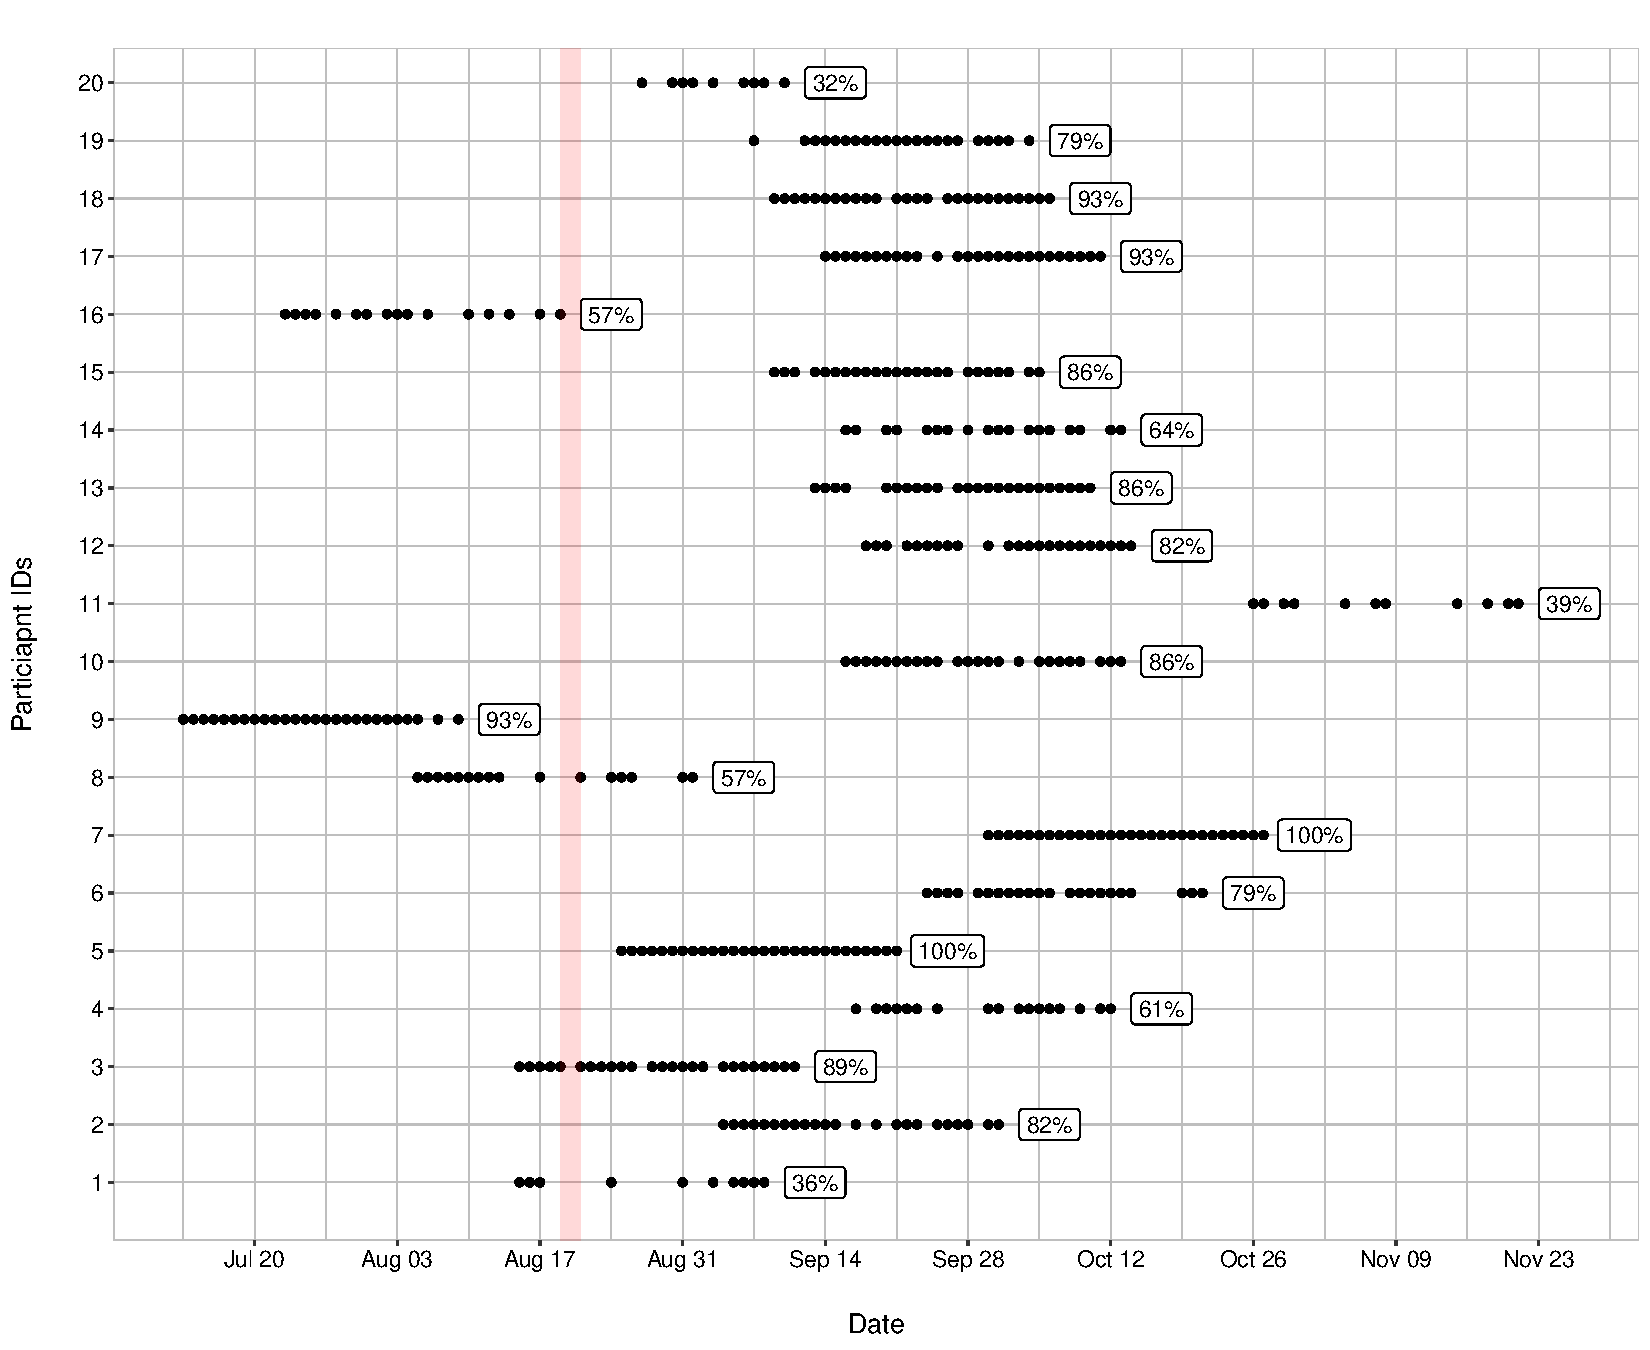
\includegraphics[clip, trim=0cm 0cm 0.15cm 0cm, width=\textwidth]{figures/engagement.pdf}
                \caption{Participants' engagement with the daily self-report of mental health and wellbeing via \acl{app}. Each dot represents an entry for the day. Annotations reflect each participant's rate of engagement calculated as the percentage of $28$ self-report sessions during the study. The red bar indicates Dialogflow's service outage on August 20th, 2020. Participants were not able to use \acl{app} on that day.}
                \label{fig:engagement}
                % \footnote{https://issuetracker.google.com/issues/165676621}
            \end{figure}
                
        During the study, $20,154$ words from $418$ daily open-ended self-reports were collected. On average, a participant's daily self-report contained $48.22$ ($\pm 30.48$ SD) words, lasting $46.96$ seconds ($\pm 31.33$ SD). The shortest self-report consisted of $4$ words while the longest contained $225$ words. Figure~\ref{fig:word-cloud} shows the words most frequently used by participants when responding to the open-ended questions eliciting expression of their emotional state. More than half ($59.33\%$) of participants engaged with the system during the evening hours of 18:00 to 21:00 as shown in Figure~\ref{fig:time_frequency}.
            
            \begin{figure}[h]
                \begin{minipage}{.48\textwidth}
                    \centering
                    %   l b r t
                    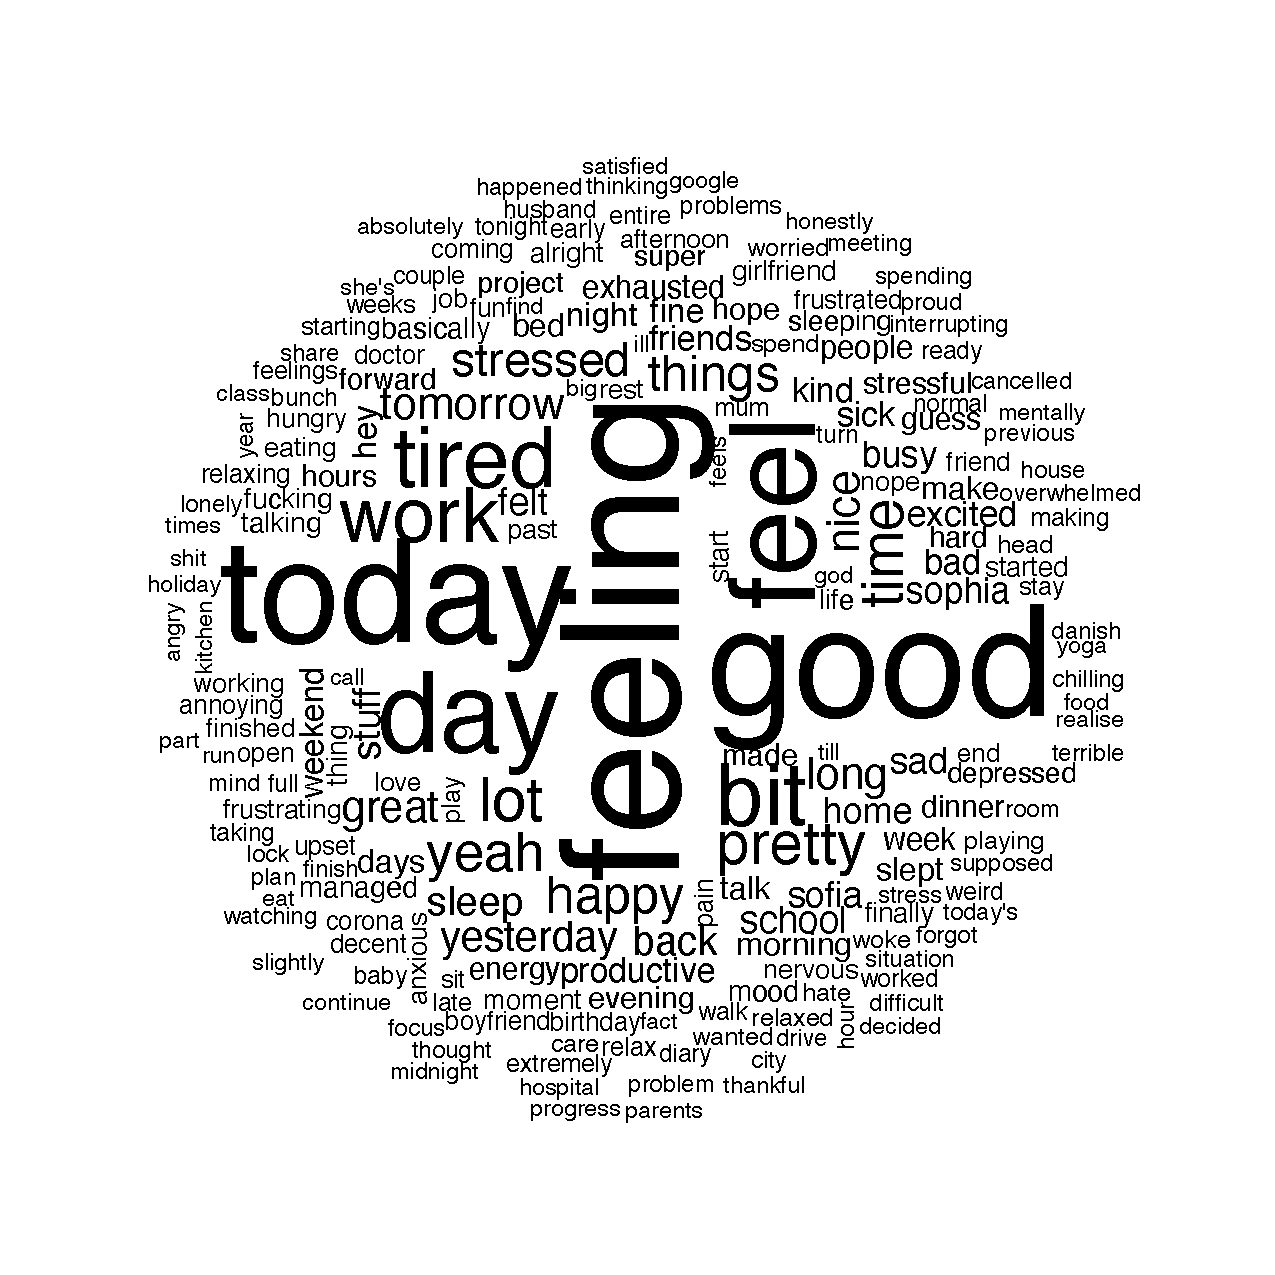
\includegraphics[clip, trim=2cm 2cm 2cm 1cm, width=\textwidth]{figures/word-cloud.pdf}
                    \caption{A word cloud generated from the participants' open-ended self-reports of their mental health and wellbeing}
                    \label{fig:word-cloud}
                \end{minipage}
                \hfill
                \begin{minipage}{.48\textwidth}
                    \centering
                    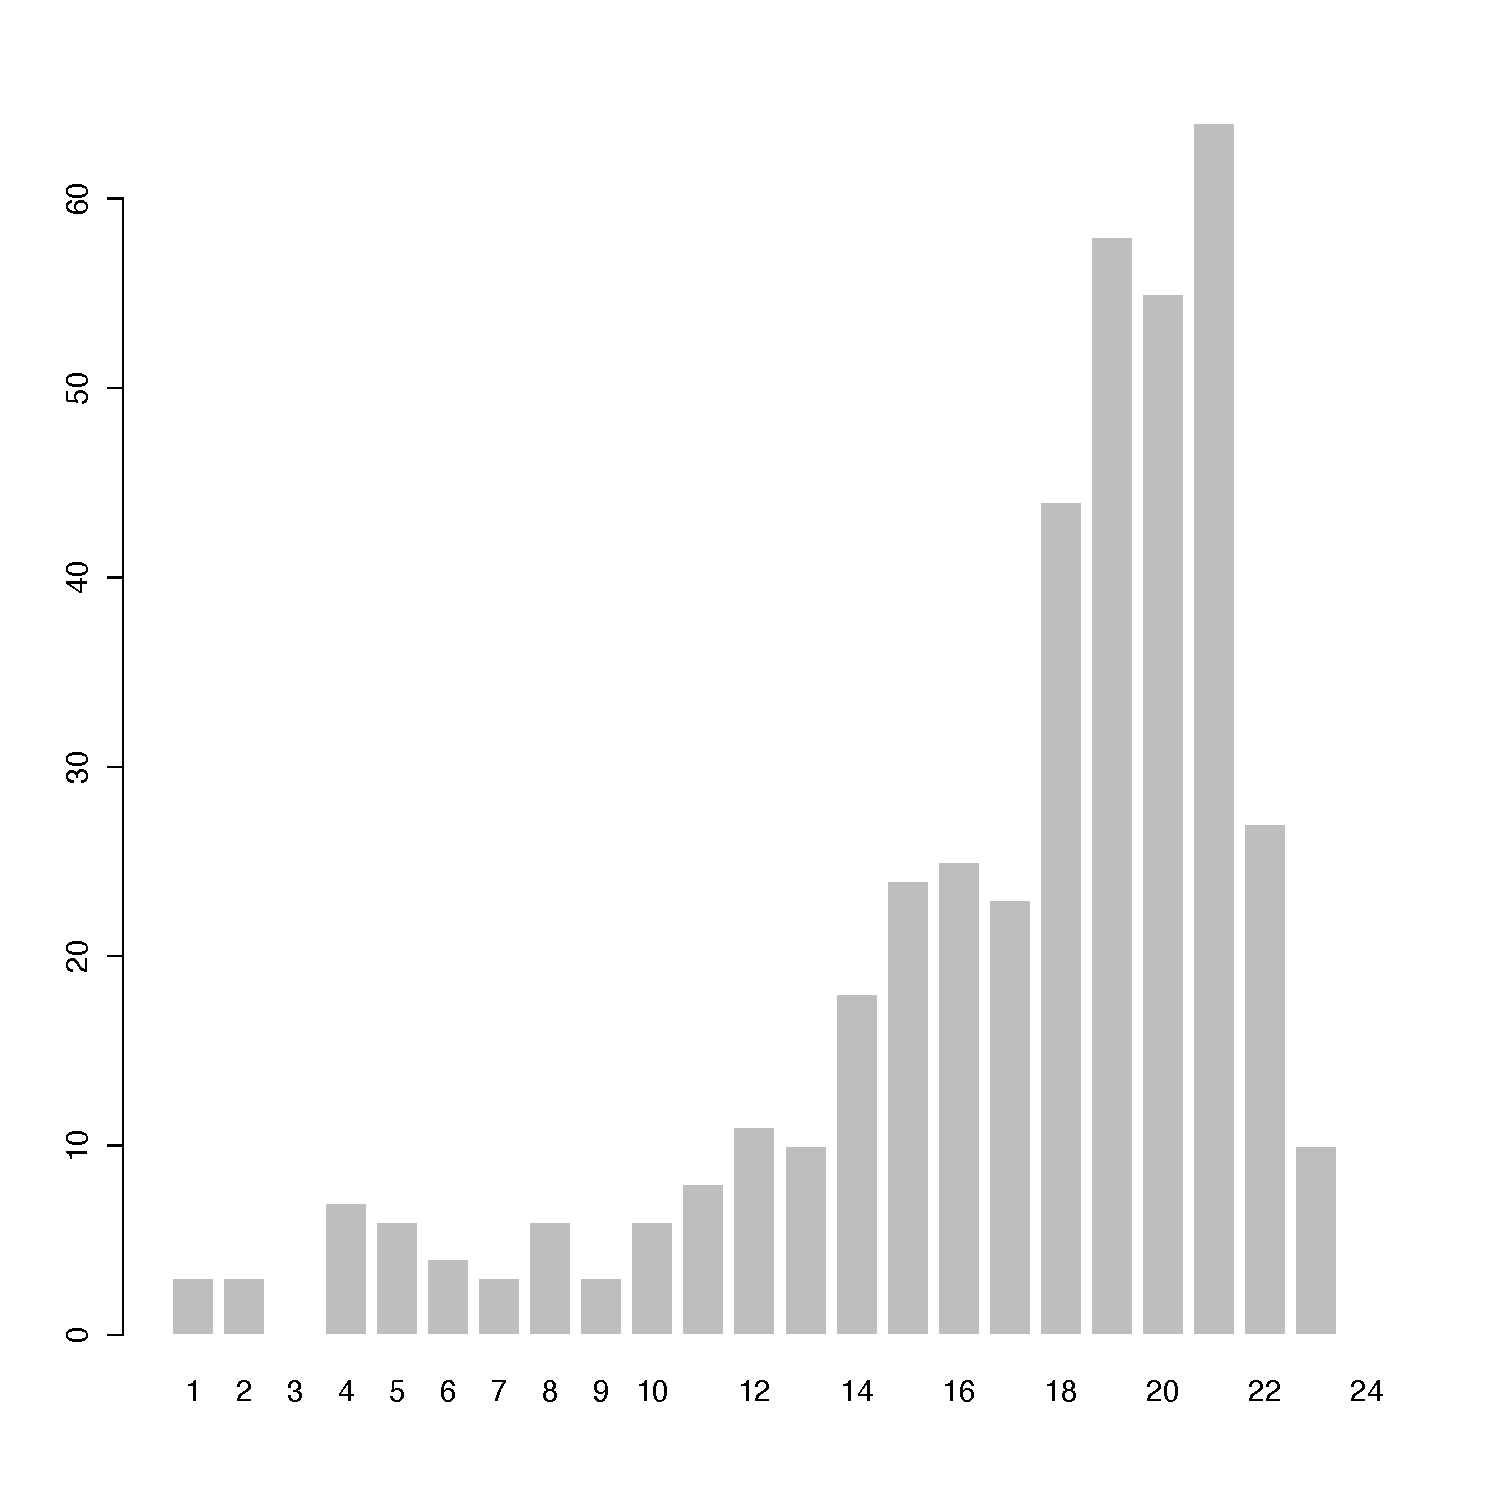
\includegraphics[trim=0cm 0cm 2cm 0cm, width=\textwidth]{figures/time_frequency.pdf}
                    \caption{Self-report frequency plotted against time of day. The x-axis represents the time of day in 24-hour format, and the y-axis self-report frequency.}
                    \label{fig:time_frequency}
                \end{minipage}%
            \end{figure}  
            
        % \subsubsection{Perceived User Experience}\label{sec:perceived_experience}
        As shown in Figure~\ref{fig:ueq-ci} participants' responses to the \ac{UEQ} questionnaire upon conclusion of the study reveal an overall positive impression of their self-report experience in terms of 
                attractiveness  ($U = 1.09, SD = 1.01 $), 
                perspicuity     ($U = 2.09, SD = 0.75 $), 
                efficiency      ($U = 0.98, SD = 0.77 $), 
                dependability   ($U = 0.74, SD = 0.84 $), 
                stimulation     ($U = 0.38, SD = 0.82 $), 
                and 
                novelty         ($U = 0.71, SD = 0.88 $). 

            \begin{figure}
                \centering
                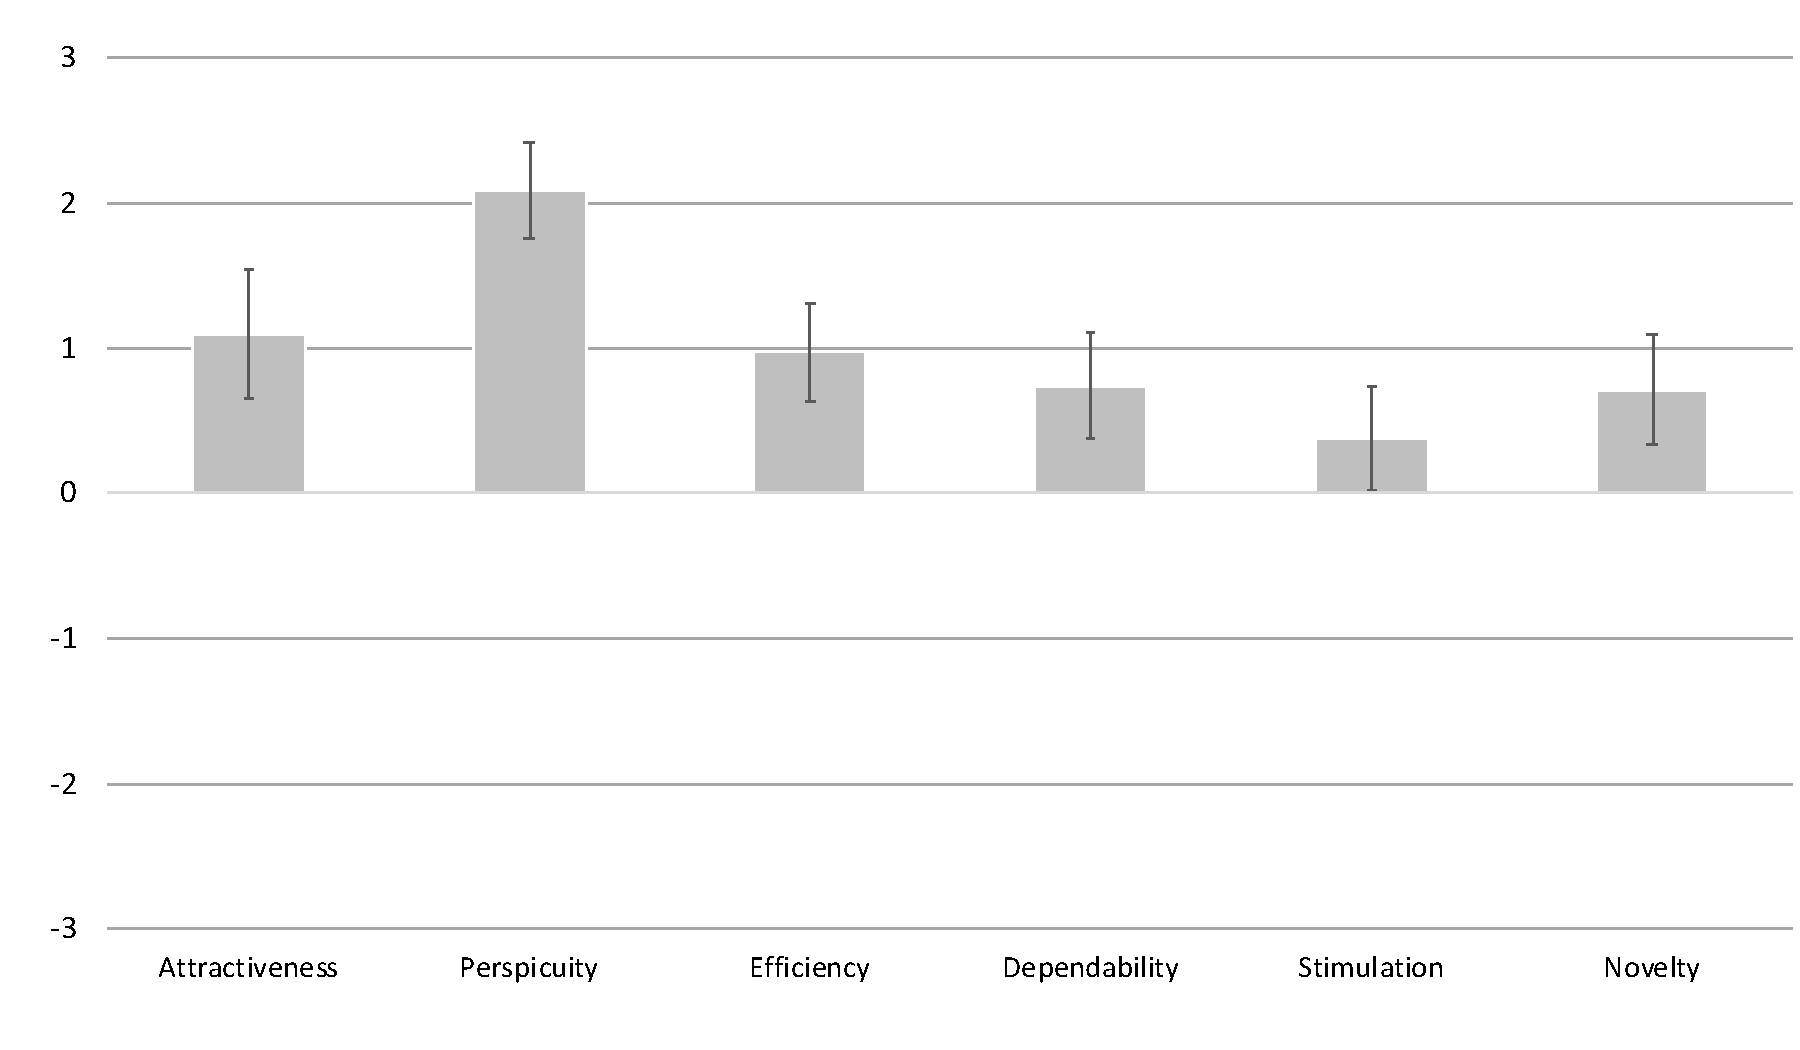
\includegraphics[width=\textwidth]{figures/ueq-ci.pdf}
                \caption{Participants' mean \ac{UEQ} score with respect to each dimension. Error bars reflect a $95\%$ confidence interval, the y-axis represents scores ranging from -3 (horribly bad) to +3 (extremely good), and the x-axis illustrates the six dimensions of the scale.}
                \label{fig:ueq-ci}
            \end{figure}
        
        These data serve as context for our thematic analysis of interviews conducted with participants following their engagement in this 4-week `in-the-wild' study; the primary findings of which we present next.
   
    % Users' experience as strongly shaped by actions taken to overcome the technological limitations of \ac{CA}s,
    % \subsection{Theme 1. A Good Experience can Enhance Engagement Despite Technical Limitations}
    \subsection{Theme 1. Engaging With \& Getting Around the Technology} % Overcoming Technological Limitations

        The theme we first discuss is one which informed all others, and stems from users' frequent comments to the need to get around the technology in order to fully engage with it. These comments relate for the most part not to choices made in the design of this particular \ac{CA} but to the more general limitations of commercially-available smart-speaker technology. These limitations undoubtedly had an impact on participants' self-report experiences, and yet the lengths to which participants went to overcome these limitations and maintain their engagement highlights the value participants saw in their use of the technology.
            
        % \subsubsection{An Efficient, Easy-To-Use and Attractive Medium of Self-Report} % UEQ related qualitative findings

        %     Many participants in this study pointed to the efficiency and convenience afforded by the smart speaker's hands-free experience as motivation for their sustained engagement with the agent;
            
        %         \begin{quote}
        %             \vspace{2mm}
        %             \textit{``I love it because it’s like an interface you talk directly to. It’s super easy to use. You don’t have to open your laptop and go to a specific page. I can just go home, open the door and talk to \acl{app}, super easy.''} [P1] 
        %             \vspace{2mm}
        %         \end{quote}
            
        %     Several participants also described how speech, as a more natural form of interaction, enabled them to express their emotions more freely and spontaneously compared to other means of self-report; \textit{``Speaking is much easier because you can just let the words flow and you don't have to think about it''} [P14]. The \ac{CA}'s tone of voice was likewise characterized by many participants as friendly, caring, and calming, resulting in a positive first impression in the context of their self-report experience; \textit{``My first impression was that I really liked her voice. She sounded very, very calming and caring''} [P7]. This was not a universal experience however, and other participants at times commented that \ac{CA}'s voice was robotic and lacked variation in tone and intonation.

        \subsubsection{Frustration, Rejection, Illusion \& Technical Limitations}
        
            Limitations described by participants include the \ac{CA}'s tendency to frequently interrupt and thereby impair their self-report experiences; due to both the \ac{CA}'s inability to recognize pauses between user utterances and the 12 second limit imposed on user responses. This would mean that participants were often interrupted in the middle of a sentence by the following question before they had completed their desired response. 
            
            % frustration / feeling of rejection / disconnect / value
            These experiences understandably proved frustrating for users, \textit{`I'm like `No bitch, you cut me off. So, shut up'\ldots''} [P9], and led to some participants quitting the conversation early; \textit{``Okay fine, that's it for today''} [P18]. Several participants compared their \ac{CA} interactions with a human-to-human conversation, and in turn expressed feelings of rejection following repeated interruptions and the inability to fully recount their emotional experience;
                
                \begin{quote}
                \vspace{2mm}
                    \textit{``I know it's not a human being. I know it's this little round little thing, but still it's like, I'm trying to be personal here and then you're interrupting me. It feels like a rejection.''} [P9]
                \vspace{2mm}
                \end{quote}
                
                \begin{quote}
                \vspace{2mm}
                    \textit{``I felt like a bit like when you talk with a friend, and they don't want to listen to you.''} [P8]
                \vspace{2mm}
                \end{quote}
                
            P8, in this example, relates their interrupted self-report experience to a conversation with a person who does not care, leading to a sense of disconnect. Similar accounts were shared by other participants who noted that it was important for them to feel listened to and cared for, despite their awareness that the \ac{CA} could not understand their emotions nor in reality `care' about what they shared.
            
                \begin{quote}
                \vspace{2mm}
                    \textit{``Of course, the software doesn't care. But, you want the illusion that it cares about you.''} [P5]
                \vspace{2mm}
                \end{quote}
            
            Many of these limitations of CA technologies are well-known and well-documented in prior literature (Section \ref{sec:ca_limitations}). What is most striking about participants' accounts as shared during this study however is the extent to which these technical limitations were recounted in emotional terms, and to which this reflects a desire by participants to relate to the technology. This theme is therefore furthermore supported by the strategies employed by participants to overcome these challenges.
  
        \subsubsection{Strategies to Overcome \ac{CA} Limitations}\label{sec:strategies_to_overcome}
        
            Participants described their development of a number of strategies to maintain their engagement;
            
            \paragraph{(i) Making Multiple Entries} % Beginning Again
        
                At the pre-study session, participants were given some insight into the limitations of the technology, and adding multiple entries was offered as a possible strategy for overcoming these challenges, should users encounter them. Only a small number of participants did adopt this strategy however; either accepting the technology's limitations and sympathizing with the CA, or interestingly, contrasting the \ac{CA}'s 12-second limitation with a human interlocutor's potentially limited capacity to listen to others;
                
                    \begin{quote}
                    \vspace{2mm}
                        \textit{``With my frustration, I took a deep breath and thought it’s just a technology. It’s in it’s starting phase - I let it do it’s thing.''} [P3]
                    \vspace{2mm}
                    \end{quote}
                    
                    \begin{quote}
                    \vspace{2mm}
                        \textit{``I guess that there's also like a limit to how, how long she can listen, like another person would also have.''} [P12]
                    \vspace{2mm}
                    \end{quote}
                
               Other participants noted that they did not find this a feasible strategy, commenting that they would lose their train of thought should they start a new session; \textit{``The problem is that you loose your momentum or train of thought when you're interrupted like that''} [P9]. P2, in contrast, compared their interactions to a human-to-human conversation and thought that it would be rude to ask \acl{app} to listen again: \textit{``when you're done talking to her and she is like `Thanks for sharing that. Have a nice day'\ldots it would feel rude to ask her again''}.

            \paragraph{(ii) Adapting One's Speech}
    
                Other participants adopted more active strategies. This included changing their natural speech patterns by stretching out their utterances, using filler words, and speaking faster or more briefly;
                
                    \begin{quote}
                    \vspace{2mm}
                        \textit{``I tried different tricks like for instance I tried to make some songs like `hmmm leeet meee thiiink' but it seems like my process was too slow for \acl{app}. So at one point, I started giving very short answers so I won’t be cut off yet could answer.''} [P1]
                    \vspace{2mm}
                    \end{quote}             
                
                Although considered effective, this approach was also certainly viewed by participants as a compromise;\textit{``My speech is a bit artificial, not very smooth, and didn't feel fluent. I had to change the way I talk to fit what \acl{app} can accept}'' [P8].
                    
            \paragraph{(iii) Preparing In Advance}
                    
                Another strategy spontaneously adopted by participants was to reflect in advance on what they desired to share with the \ac{CA}. P16 for example, recounted how they would divide their response into three parts to match the design of \acl{app}'s dialog flow:  
                
                    \begin{quote}
                    \vspace{2mm}
                        \textit{``I realized, okay two sentences for the first question, two sentences for the second question, and one sentence for the last question. Just five sentences overall.''} %[P16]
                    \vspace{2mm}
                    \end{quote}   
                
                Interestingly, some participants commented that this process of formulating their thoughts in advance in itself helped them to reflect on their day. P11 viewed this process as `meditative,' commenting, that \textit{``it helps you organize things in your head\ldots It's like `you time', you know, I believe it helps you clear your mind''}. P6 compared the experience to composing a concise diary entry which served to focus their reflections; \textit{``It's not just three pages of how I saw something nice and I had a nice cup of coffee\ldots It really is an emphasis on three things which really matter to me''}.
                
                Although for some participants such tactics led them to feel their responses were increasingly shallow, \textit{``She expects an answer in few seconds, so I'll be like, `tired', `decent', `not sure'. So in that sense, the answer might be a bit less thought out''} [P2], others showed a surprisingly significant willingness to adapt, at times expressed in overtly human terms;
            
                    \begin{quote}
                    \vspace{2mm}
                        \textit{``I started thinking about what I want to say before I called her up. Normally, when people talk about feelings, they need space and time for pauses. I knew my \acl{app} friend could not really do that. So we had to do it on her terms.''} [P7]
                    \vspace{2mm}
                    \end{quote}  
                
            A number of participants spoke to their increased capacity to adapt to the technology's limitations over time, despite the undoubted impact on their experience; \textit{``It was kind of hard in the beginning as she is really sensitive to pauses and doesn't give you any space to think. But my brain adapted that really quite quick''} [P7]. This willingness to adapt can only be interpreted in light of the value users associate with their interactions with the technology -- which, despite these limitations, appears to be closely related to their perceptions of the agent itself, as reflected in our second theme.

    \subsection{Theme 2. ``Sometimes All You Need is Someone Who Listens''}
    
        Engaging in the self-report of mental health and wellbeing by any means is an exercise in vulnerability. And many participants spoke to this effect, commenting how they would refrain from sharing their emotions even with close friends and family due to the social stigma attached to their illness. P7 and P14 noted the need to think about the potential repercussions of disclosure, listeners' reactions, as well as the potential for others to demonstrate disinterest in the subject, each of which demotivated their sharing of emotion;
    
            \begin{quote}
            \vspace{2mm}
                \textit{``You know, my dysphoria (\acs{PMDD}) often makes it so that I think that I'm a bother to people, like `it's really annoying to listen to you bitch'\ldots''} [P7]
            \vspace{2mm}
            \end{quote}  
    
        Another barrier to self-expression recounted by participants pertained to the potential for listeners to become pre-occupied with trying to understand their emotions in depth, requiring them to repeatedly explain what they are experiencing, when most of all they wished simply to be heard; \textit{``When you say you feel sad and empty, you don't really want the focus to be on describing how emptiness feels. You just want to say, `I'm feeling sad'\ldots''} [P6]. Strikingly, participants also frequently commented on their struggle with listeners' keen desire to `solve' their problems rather than listening to them. They explained that they usually do not require a solution to their problems, and due to the chronic nature of their conditions, often know how to cope with their situation and ongoing mental state; 
        
            \begin{quote}
            \vspace{2mm}
                \textit{``Sometimes all you need is someone who listens than have an answer\ldots because there's not necessarily anything to solve, you just need someone to share your thoughts and feelings so that you are not alone.''} [P2]
            \vspace{2mm}
            \end{quote}  
        
        This desire to be listened to, rather than to have their problems solved, goes some way towards explaining the value users saw in this particular \ac{CA} implementation, although interpretations and perceptions of \ac{CA} itself were strikingly diverse;
        
        \subsubsection{\ac{CA} as Good Listener}\label{sec:good_listener}
        
            Throughout the interviews, participants' comments echoed a desire for \textit{``emotional support instead of emotional counseling''} [P7], a role for which \acl{app} was often appropriated, as `someone' who made them feel heard. For many participants, therefore the \acl{app} was simply a good listener, who allowed them to express their emotions freely; 
            
                \begin{quote}
                \vspace{2mm}
                    \textit{``It sounds a bit stupid to say but I could say that I'm glad someone listens, except you know there isn't actually someone that listens. But it feels like it.''} [P2]
                \vspace{2mm}
                \end{quote} 
                
                \begin{quote}
                \vspace{2mm}
                    \textit{``She is a good listener. Sometimes a listener is exactly what you need in a situation like that.''} [P6]
                \vspace{2mm}
                \end{quote} 
                
            Participants valued the non-judgmental nature of conversations with \acl{app} which neither provided unwanted solutions nor meant that they had to worry about potential judgment and repercussions for sharing their feelings; \textit{``Since I knew \acl{app} doesn't mind, I felt it in some instances in a twisted way, I felt like she cared, like she was always there no matter how negative or positive I was feeling.''} [P7]. They furthermore appreciated \acl{app}'s compassionate feedback and mentioned that it would provide a sense of comfort and empathy when feeling depressed;
            
                \begin{quote}
                    \vspace{2mm}
                    \textit{``When you have a diagnosis like this, you know that only talking doesn't make it go away, but sometimes getting assurance `Okay, it's okay to feel, it's okay to experience what you experienced', that helps a lot.''} [P6]
                \vspace{2mm}
                \end{quote} 
            
        \subsubsection{\ac{CA} as Machine Companion} % Coach / Counsellor ?
            
            Other participants employed a vocabulary of companionship when describing \ac{CA}, associating the technology's value with its ability to fill a felt gap in their social interactions;
            
                \begin{quote}
                \vspace{2mm}
                    \textit{``When you are depressed, your social circle tends to restrain more and more. So, you’ve less opportunity to talk to someone. I felt like I was talking to someone even though \acl{app} is not very smart. Just because of this feeling, I think it is very useful for people with depression.''} [P1]
                \vspace{2mm}
                \end{quote} 
            
            For some participants, the \ac{CA}'s value, therefore stemmed from its constant availability; \textit{I do have friends to talk to. But a friend could be busy. When you need to talk it out, it’s in your reach even though it’s a machine'' } [P5]. Others spoke of the \ac{CA} as also more approachable and trustworthy --- a perception of the \ac{CA} as a harmless machine meaning that it could not turn against them no matter what they shared;
            
                \begin{quote}
                \vspace{2mm}
                    \textit{``I have massive trust issues. I grew up thinking that whoever you tell anything, they will use it against you. But, since I know that \acl{app} is a machine, she doesn't really think that much of herself and she's just there sitting on my table. That kind of makes it a little bit more approachable.''} [P7]
                \vspace{2mm}
                \end{quote} 

            And yet, for P4, talking to a \ac{CA} about their emotions could equally serve to make them feel lonely, given that the \ac{CA} could not `truly' understand their feelings; \textit{``Sometimes she made me feel a bit lonely, somehow, because you're just reminded that you're talking to a machine, who has no capacity to understand what you're actually feeling\ldots something that kind of tries to mimic a human being but it's not convincing''}.

        \subsubsection{\ac{CA} As Human} % Friend?
        
            Other participants went to greater lengths to personify the \ac{CA}, with both positive and negative implications and associations.

            % +ve personification
            Participants with positive perceptions of their self-report experiences tended to personify the \ac{CA} as a friend, therapist, or talking diary. Although noting their awareness that the \ac{CA} was not human, participants would often comment that the anthropomorphic characteristics of the \ac{CA} granted them the impression of a conversation with a person. P10, for example, who personified \acl{app} as a friend, commented \textit{``I think it's the whole, having a voice and having a name, I keep referring to it as her instead of it, even though I'm aware that it's a system and not a person''}. 
            
            P14 personified \acl{app} as an older friend and mentioned that although she could also be their age, \acl{app}'s voice made them think of someone older; \textit{``Its more like an older friend. I mean I'm also quite young, I'm 25 so maybe that's why? Maybe it's also the voice that reminds me of someone a bit older than I am''}. P15, on the other hand, viewed the \ac{CA} as a `talking diary' and compared their self-reporting practice to talking to their dog; \textit{``I compare \acl{app} to my dogs. Because a lot of the times, especially when I was growing up, if I was upset I went outside, sat down and talked to my dog who had no freaking clue what I was talking about, and it made me feel better''}.
            
            % -ve personification
            In contrast, participants with negative perceptions of their self-report experiences personified \acl{app} as an elderly woman, an uncaring friend, and a teenager trying to act grown-up. Referring to the \ac{CA}'s tendency to frequently interrupt her mid-sentence, P9 personified the \ac{CA} as a friend who does not care; \textit{``It's kind of like, you know, that friend who like sits with the phone when you try to talk about something deep, like `Okay fine, just say you don't want to listen to me'\ldots''}. Likewise, P3 personified the \ac{CA} as an impatient old lady, an impression informed by the 12-second response limitation and tone of voice; \textit{``\acl{app} is like a very impatient woman and she’s probably quite old. She’s very monotoned, there’s no variation''}.

            % Personification and self-reporting behavior
            These various personifications also shaped participants' responses to the agent, including their self-reporting behaviors. A positive personification of the \ac{CA} motivated P6 to find and share positive emotions even when negative ones were abundant; \textit{``You feel like, `Oh, I'm talking to someone and I don't just want to be negative. I want to say something positive'.''} Whereas, for P9, a negative perception of the agent led them to vent their frustrations directly to the device; \textit{``Sometimes I guess it took my emotions out. 
            %Sometimes I was yelling at her, telling her to fuck off. 
            It was probably not her causing the reaction, but because I was annoyed about something, and then I took it out on her. Sorry \acl{app}''}.
      
        \subsubsection{\ac{CA} As Blank Slate} % Null
     
            Finally, a number of participants spoke of emotional venting and self-talking as useful practices enabled by the smart speaker device. These accounts reflect interpretation of the \ac{CA} as a blank slate. P11 and P14 considered self-reporting via \ac{CA} a self-talking exercise, and stated that doing so helped them to clear their mind ~\cite{callicott2003effects,kendall1991guiding,treadwell1996self}. As P14 noted:
            
                \begin{quote}
                \vspace{2mm}
                    \textit{``Once you say stuff out loud, it just changes how you think about certain things\ldots when I have them in my head, it just sounds like they are super important. If I just talk out loud, then suddenly it becomes less important and I realize that they're just thoughts and they're not really like who I am.''} %[P14]
                \vspace{2mm}
                \end{quote} 
            
            Emotional venting has likewise been regarded as an effective means of finding relief by releasing strong or repressed emotions~\cite{bennett1991irrationality, tonnaer2020explosive, leslie2008boxing}, a practice on which P8 commented;
            
                \begin{quote}
                \vspace{2mm}
                    \textit{``I almost see it as, you know, when you get super upset, you go out and scream, you go very far away and you just scream at the wind, cows or whatever. And you know that you're never going to get anything back, like, no one is going to respond to you, but it feels good to just express.''} %[P8]
                \vspace{2mm}
                \end{quote} 
            
            These various perceptions of \acl{app} suggest the value of different framings and implementations of mental heath agents, and multiple paths forward for their future design for varied yet valuable purposes. The prevalence of personification in itself furthermore underlined the extent to which participants perceived self-report as a socially-contingent practice.        

    \subsection{Theme 3. Self (Report) is Social}
    
        While all forms of self-report, and indeed human behavior, are to one degree or another socially-contingent in nature, participants' experiences of \acl{app} in particular revealed a diverse variety of social associations. Many of these accounts stem, at least in part from the spoken nature of the interaction itself, and in turn its more open nature.

        \subsubsection{A Private Practice Rendered Social} % Social influence in self-reports
            
            Eight of the twenty ($40\%$) participants in this study mentioned that they engaged with \ac{CA} in an open environment (e.g., a co-living space) where the presence of others' was likely to have an effect. And yet this was not the only way in which social considerations were seen to manifest. The choice of a number of participants to make their self-reporting a private practice was also informed by their social circle's perception of the \ac{CA}, as well as their relationships to their loved ones.
            
            The self-report of mental health and well-being is most typically a private practice, due at least in part to the social stigma attached to many mental health conditions, and the potential lack of privacy when engaging with a \ac{CA} therefore creates a unique self-reporting context. Participants P17 and P20 commented that it felt `weird' and `awkward' to talk to \acl{app} when other family members were around; \textit{``It felt a bit weird talking to a speaker and was especially weird when my husband was home. It was unnatural in general but especially when I had someone else listening at the same time''} [P17]. For P4, this experience was awkward because it created confusion when their partner did not know that they were talking to the \ac{CA}:
            
                \begin{quote}
                \vspace{2mm}
                    \textit{``Talking to \acl{app} is little awkward because because if my boyfriend wasn't aware of what I was doing, He's like, `What? `Do you want something from me?'\ldots like `No no. I'm talking to the device'. Yeah, `I'm talking to this other thing in our house'.''} %[P4]
                \vspace{2mm}
                \end{quote} 
            
            P6 shared that although it was also strange for them to talk to \acl{app} initially, it became natural due to their partner's support -- serving as an interesting example of the implicit value of such a technology in providing an opportunity for others to demonstrate care;
            
                \begin{quote}
                \vspace{2mm}
                    \textit{``At first, I felt like this is something personal. Like, this is something I should hide, like a diary under the pillow or something. But, well first of all, my husband has been really supportive and he is like, `Remember your \acl{app}, Remember to talk to her'. So it became more natural to talk to her.''} %[P6]                
                \vspace{2mm}
                \end{quote} 
            
            Of course, reporting practices varied among participants, as intended by a study designed to allow users to appropriate the technology as they saw fit. P11 noted that they were comfortable sharing their feelings in the presence of others, \textit{``I don't mind\ldots sharing these things with my friends, or anyone to be honest''}, whereas P3 commented that they refrained entirely from self-reporting when friends were around; \textit{``I’d have friends over so during those times, I didn’t log a diary -- You don’t want to let everyone know about deep personal life.''}
  
        \subsubsection{A New Member of the Social Circle} % Social perception of \ac{CA} self-reports
        
            Other participants went further, and spoke of \acl{app} as entering into their social circle. A number of participants commented that their social circle held a positive view of the \ac{CA} and supported the idea of talking to \acl{app} about their emotions. P1's partner, for example, told P1 that \ac{app} could help them when they were feeling down; \textit{``My boyfriend told me that maybe I should use \acl{app} when I was down. He told me that I shouldn’t be closing myself to the world, I should be talking. He said it might be useful.''}. 
            
            P6 spoke openly about the study with friends and family, and described their friends as very curious about the technology, which quickly became a topic of conversation in their daily lives;
            
                \begin{quote}
                \vspace{2mm}
                    \textit{``I remember a friend who said `so how's it going with \acl{app}?', and they started joking and like `So when is she going to tell you about her'? It's quite interesting how she became this little person in my life somehow''} %[P6]          
                \vspace{2mm}
                \end{quote} 
            
            P6 continued that their father was equally excited about the technology and shared that he had in turn also expressed an interest in purchasing a smart-speaker, as a potential means of addressing loneliness. However, they also wondered whether their father would be able to set up the device;
            
                \begin{quote}
                \vspace{2mm}
                    \textit{``I talked to my dad, he was really interested. 
                    He's like how does someone put a voice in this tiny box? like he doesn't understand it's just code and such. I asked him if you would buy something like this and he said yeah he probably would because he's also alone a lot of the times. But he also said, `if I have to use it with apps and phones, I can't figure out how to do with them'\ldots ''} %[P6]
                \vspace{2mm}
                \end{quote} 
            
            P18's friends similarly thought that \acl{app} was `cool' and expressed its potential to support mental health and wellbeing. Their partner commented however that, although such a system could help those particularly isolated, it would not be able to replace a more human connection;
            
                \begin{quote}
                \vspace{2mm}
                    \textit{``My boyfriend is a therapist himself and he said that, that might be smart. It could do something for very very very lonely people. They could feel like, `Well, there's someone who is interested in my day'. But we also talked about like we don't think an artificial intelligence can ever replace of a real life person''} %[P18]
                \vspace{2mm}
                \end{quote} 
            
        \subsubsection{An Influence On Close Personal Relationships} % Self-reporting via \ac{CA} and social relationships
        
            Finally, and perhaps most surprisingly, a number of participants spoke of the influence of \acl{app} on their intimate and personal relationships. Several noted that openly describing their emotions to the \ac{CA} also led to conversations with their partners, and served to strengthen their relationships.

            P4 commented that after hearing her response to the fortnightly \ac{WHO-5} questionnaire, her partner realized for the first time just how she had been feeling during those two weeks; \textit{''When he heard me responding to \acl{app}, he was like, `oh so this week is that shit? I didn't know'\ldots''}, creating a `different situation', \textit{``an intervention in your life where you're like, so this is how you're actually feeling''} despite the fact that \textit{``of course, we see each other every day, we live together. I do tell him if I'm tired or mad or whatever and try to keep him in the loop about my moods. But it's also just like sometimes you're not aware of it yourself''}.
            
            This potential of the technology to shape the social fabric of a household was reflected in several other participants' comments. P6 mentioned that their mental condition could make it hard for them to explain exactly how they are feeling, and that their tone of voice when speaking to \acl{app} therefore became the medium by which their significant other could best understand how they are actually feeling;
            
                \begin{quote}
                \vspace{2mm}
                    \textit{``Sometimes I will talk to her and not like I said anything specific but more like he [P6' husband] could feel from, how I was talking to \acl{app}, my tone of voice. Some days he would peek his head in and be like, `Do you want to talk about anything?. Are you okay?', because I can be feeling extremely bad, but I'll look Okay.''}
                \vspace{2mm}
                \end{quote} 

            P14 spoke of a moment of realization during which her and her partner noticed that although they talked about their daily activities, these conversations did not necessarily reflect their feelings. 
            
                \begin{quote}
                \vspace{2mm}
                    \textit{``My boyfriend does not share his emotions very often, neither do I. 
                    %You always ask like `How was your day?' but then it's always a bit vague. 
                    So sometimes when I was talking to \acl{app} and he (P14's boyfriend) noticed that I had some different feelings which he wasn't aware of. It was quite good in that way. Now we are speaking more about feelings. 
                    %Now we ask `How are you feeling today?' and it's not only good but then 
                    We also have more details about how it is going. 
                    %I think it's very important.
                    ''}
                \vspace{2mm}
                \end{quote} 
                
            Many participants' comments therefore reflected an open and welcoming attitude towards \acl{app}. And yet, this did not preclude attention to questions of privacy and security, as our final theme highlights.

    \subsection{Theme 4. Personal Privacy \& Data Security}\label{sec:privacy}
    
        In line with prior research~\cite{lau2018alexa}, participants' engagement in self-report was also shaped by their perceptions of personal privacy and data security. Although open to interpretation as pragmatic in nature, the implications of these concerns were not straightforward, as this theme highlights.   
        
        \subsubsection{Away From Prying Eyes \& Ears}\label{sec:eavesdropping} % Eavesdropping
        
            A number of participants recounted privacy concerns stemming from their own and their wider social circle's perception of the technology. The concern most-often shared related to the potential for the smart-speaker device to continuously listen and record conversations, even when not activated. In order to protect their privacy, participants described either turning off the smart speaker's mic or unplugging the smart speaker entirely. Participants P12 and P14, for example, both commented on the potential of the technology itself to serve as a source of anxiety, and subsequently chose to keep the microphone off at all times, only turning it on when speaking to \acl{app}: \textit{``I felt a bit paranoid so I was like turning the speaker off''} [P12].
   
            A small number of participants commented on their resignation from engagement with the challenge of navigating many questions of privacy, due to a perception that it was broadly impossible to avoid pervasive collection of their data. P16, for example, mentioned that they did not mind sharing their data as long as they got something in return: \textit{``I'm not really concerned about privacy because I cannot stop them (tech companies) from collecting the data. But if I'm sharing something, I need something in return. For example, I really like that every month Google sends you  a timeline and gives you how many kilometers you have walked''}.
            
        \subsubsection{Hands Off Our Data} % Data security
            
            In addition to their concerns regarding potential eavesdropping, participants expressed an interest in knowing and closely controlling how their data would be handled, citing understandable fears that their data might be shared with a third party or become publicly available. 
            
            Although appropriate limitations on the use of patients' data were carefully explained both in-person and within participant materials, these privacy concerns understandably had an impact on certain participants' self-reporting practices. P9 commented that they \textit{``probably held back, a great deal. Because of the whole, I know that it's not ending up in cyberspace for anyone to see but there's still that thought that is a bit more out of my control than if I have it in a physical diary''}. Despite describing herself as an open book, P18 also commented that knowledge of the research team's access to her transcripts led her to refrain from fully recounting her mental states, \textit{``I knew that you would get the transcript of what I told her. Now, I'm not really a private person and I'm pretty much an open book, but I did refrain from saying stuff that I would have said if I knew you wouldn't be able to read it''}.
                      
            These concerns are not new, yet are particularly important to consider, and of particular ethical significance, in the lives of this population group, whose involvement in this study and engagement with this technology consisted of a vulnerable exercise requiring high levels of social trust and personal courage. 
        
    % \subsection{Theme 5. Action Items to Improve Conversational Interaction for Mental Health Self-Report }\label{theme:design_recommendations}
    \subsection{Theme 5. Designing for Conversation \& Reflection}\label{theme:design_recommendations}
    
        Many participants spoke of the value of the technology as allowing them to fully express their emotions, and yet also as one of the ways in which the system was currently most limited. Additionally, they highlighted the potential need to reflect on their self-reported data and discussed ways to enable this.
        
        \subsubsection{Designing for Conversation}\label{sec:improve_design}
            
            Participants made several design recommendations to improve the \ac{CA}'s conversational skill, and allow users to express their emotions more fully.
            
            \paragraph{(i) Varying More Often}
            
                Participants recommended incorporating greater variation in questions, including voice characteristics (e.g. tone and intonation), and randomizing their presentation more often so that the questions did not feel repetitive;\textit{``No one's going to ask you the same kind of question in the same way with the same intonation every time. So having a few different questions and rotating them would be better''} [P18]. In contrast however, P6 noted that the repetitiveness of certain questions provided consistency in interaction which they found important; \textit{``What's really important when you suffer from a condition like schizophrenia is consistency \ldots And in that regard, I almost find a sort of comfort in \acl{app}. She is like an anchor, which you can use to ground yourself, because she always says the same thing''}.
            
                Participants perceived the fortnightly \ac{WHO-5} questionnaire as a useful addition of variety to the daily open-ended questions; \textit{``I was happy when those questionnaires came up - it was something different at least''} [P5], and several suggested also adding more discrete questions to the conversation design; \textit{``She could toss in some of that once in a while that wouldn't actually be bad''} [P4]. While many agreed that closed-ended questions can be more efficiently answered, P9 and P10 also interestingly noted that responding to the discrete questions according to a pre-defined scale made them feel more like study subjects; \textit{``You feel a bit more like a study subjects like okay `How do you feel from 1 to 10?', it's like `okay 1\ldots 5\ldots 3'\ldots''} [P9]. 
                
            \paragraph{(ii) Probing Further}
                
                Participants suggested probing their responses further to engage them in a more `natural' conversation. They stressed that the \ac{CA} does not need to understand everything but could employ strategies to support a richer conversation. P20 provided an example; \textit{``For e.g., If I say, `It was a very busy day, very overwhelming', then she could ask like, `How did you deal with that?' `How could you improve?', So it’d be best if there was an \ac{AI} which could pull out some key words and follow up on the basis of those keywords''}.

            \paragraph{(iii) Guiding More}
            
                Many participants also suggested alternate conversation designs. P18 commented, for example, that when depressed, they would tend to have negative thoughts all the time, and would appreciate a conversation that encourages them to talk about something positive in their lives; \textit{``She could ask me like, `Can you tell me a positive thing that happened to you today?' I can always tell you about bad things happening in my day. It would be better if I was turned away from that a little bit''} [P18]. P15 shared similar views but argued that the conversation should delve into both positive and negative emotions, including the reasons behind those emotions. P12 and P19 likewise advocated enabling users to select the topic of the conversation, envisioning a set of topics from which users could choose, allowing users to lead the conversation and reflect more deeply on their emotions; \textit{``If it had a certain set of questions for different topics that would help people reflect a lot more and having to be the one leading the story through the entire way''} [P19].

        \subsubsection{Designing for Reflection}\label{sec:reflection}
        
            The practice of reporting entails reflection - a point a number of participants highlighted - and the design of a self-report experience might therefore equally be construed as structuring a practice of reflection. Participants' comments for improvements in turn pertained not only to the current conversational design but also to the potential to support further reflection on their own reported data. Many participants discussed the need for a visual tool as a mobile or web app displaying the trend of their emotional wellbeing for self-reflection, arguing that it would be the easiest means of searching and examining their information.
                   
            Others however, also raised the possibility of adapting the voice interface to support reflection. P14, for example, reflected on their use of a mobile app for this purpose and mentioned that they often ignored the data shown by the app. Via verbal reflection, they stated, it would feel more like confronting a problem, which they would find more meaningful than visually examining their data; \textit{``If someone is telling me like `Hey man, I've noticed that the last couple of days you have been really stressed out, is there anything wrong?' or `What's going on?'. It's more confronting\ldots and I think that gives me way more like meaning than if I just see that in the app''}.
            
            For P15, reflecting via \ac{CA} could also provide value by granting them more scope to disagree with advice provided. Compared to the potential for confrontation with friends, family, and therapist, they felt this approach could better support behavior change; \textit{``I would be way more likely to listen to a machine because even if it tells me something like a recommendation or tells me what to do, if I don't want to do it, I'm not gonna do it''}. Participants discussed different ways in which the \ac{CA} could present data verbally for users to reflect upon. They debated whether the \ac{CA} should automatically announce the data every session or on-demand. Those who supported automated voicing of the data recommended that the information should be announced casually at the end of the session. Others cautioned that the idea of presenting the data without users' request could prove intrusive depending upon the user's mental state; \textit{``It's kind of a double edged sword, because it can be intrusive if you don't want it. If you don't want any feedback, and then \acl{app} tells you, `oh it's been really bad the past three weeks.' That's the last thing that you want to hear''} [P8].
            
    We conclude this paper with further reflection on these themes and their implications for design.

% UNUSED NOTES
% \subsection{Summary of the Qualitative Findings}\label{sec:enablers_barriers}
% elow, we summarize the key findings from our thematic analysis of the interviews.
% Table~\ref{tab:theme_summary} summarizes the five major themes from our qualitative analysis of the interview data.
% and outlines users' perceptions of \ac{CA}s for the self-report of mental health, including enablers and barriers to their use.
% \begin{itemize}
% \item\textbf{\ac{CA} as an engaging medium for the self-report of mental health and wellbeing.} Overall, participants in this study perceived \ac{CA} as an efficient, easy to use and attractive medium self-report despite its technical limitations. Although some participants expressed their self-reporting experience via \ac{CA} as frustrating and feeling of rejection, many appropriated the system by applying tactics such as making multiple entries, adapting one's speech, and preparing in advance.
% \item\textbf{``Sometimes All You Need is Someone Who Listens.''} Due to the social stigma attached to mental illnesses, many participants in this study expressed that they refrained from sharing their emotions even to close members of their social circle. Their desire to be heard was perceived as fulfilled by \acl{app}, which led them to personify the \ac{CA} as a good listener, companion, and blank slate.
% \item\textbf{Self (Report) is Social.} Participants shared the personal and interpersonal effects of using the \ac{CA} for the self-report of mental health and wellbeing. For participants living in co-living spaces, the typically private practice of self-report became social. Some described the \ac{CA} as a new member of their social circle, while others mentioned its positive influence on their close personal relationships.
% \item\textbf{Personal Privacy \& Data Security.} Participants were mostly concerned about the possibility of smart speakers eavesdropping even when they are not activated. They either turned off the smart speakers' mic or unplugged the device entirely to protect their privacy. Participants expressed that the transparency about the data practices in the study enabled them to take necessary actions to use the system at their own discretion.
% \item\textbf{ Participants’ Design Recommendations.} Based on their self-reporting experiences via \acl{app}, participants recommended improving \ac{CA}'s conversational skills by varying the questions more often, probing on their responses and guiding the conversation, and providing space for reflecting on their self-reported data.
% \end{itemize}
% \begin{table}[h]
    \footnotesize
    \centering
    \caption{Summary of the themes as users' perceptions, enablers and barriers of using \ac{CA}s for mental health self-report}
    
    \begin{tabular}{p{3.20cm} p{4.65cm} p{4.65cm}}
        \toprule
        \textbf{Themes (Perceptions)}	& \textbf{Enablers}	& \textbf{Barriers}\\
        \midrule
            
            \begin{itemize}[leftmargin=0em]
                \item[] 1. Engaging With \& Getting Around the Technology
            \end{itemize}   
        & 
            \begin{itemize}[leftmargin=1em]
                \item Speech as an efficient and easy medium of self-report
                \item \ac{CA}'s friendly, caring and calming voice
                % benefit = burden-free self-report
            \end{itemize}
        &  
            \begin{itemize}[leftmargin=1em]
                \item \ac{CA}'s technical limitation constraining the length of open-ended self-report
                % risk = adding up unwanted stress    
                \item Robotic voice of \ac{CA} due to lack of variation in its tone and intonation
                % risk = disengagement
            \end{itemize}\\ \rowcolor[gray]{.95}  
            

            
            \begin{itemize}[leftmargin=0em]
                \item[] 2. ``Someone'' (or something) ``who listens''
            \end{itemize}
        & 
            \begin{itemize}[leftmargin=1em]
                \item \ac{CA}'s anthropomorphic characteristics
                \item \ac{CA}'s compassionate feedback 
                \item Continuous availability 
                % benefit = Repercussion-free and non-judgmental venting of emotions
                % benefit = \ac{CA} as a companion
                % benefit = providing sense of comfort and empathy
            \end{itemize}
        &  
            \begin{itemize}[leftmargin=1em]
                \item \ac{CA}'s inability to understand users' feelings
                % risk = Feeling of loneliness because \ac{CA} is just a machine
                % risk = \item Negative personification leading to vent their frustration on \ac{CA}
            \end{itemize} \\
            

            
            \begin{itemize}[leftmargin=0em]
                \item[] 3. Self (Report) is Social
            \end{itemize}
        & 
            \begin{itemize}[leftmargin=1em]
                \item Support from users' social circle
                % benefit = \ac{CA} as a medium to share emotions with the loved ones
                % benefit = Positive influence on users' intimate and personal relationships
            \end{itemize}
        &  
            \begin{itemize}[leftmargin=1em]
                \item Users' social situation
                % risks = Talking about feelings without privacy is strange, weird and awkward
                % risks =  Talking to \ac{CA} in co-living spaces creates confusion
            \end{itemize} \\ \rowcolor[gray]{.95}  
            
            
    
            
            \begin{itemize}[leftmargin=0em]
                \item[] 4. Personal privacy and data security
            \end{itemize}
        & 
            \begin{itemize}[leftmargin=1em]
              \item Privacy resignation 
              \item Ethics and regulation
            \end{itemize}
        &  
            \begin{itemize}[leftmargin=1em]
                \item Users' privacy (eavesdropping) concerns
                \item Distrust of \ac{CA} data security
                % risk = Paranoia and anxiety due to the concerns
                % risk = data quality (they held back on their self-report)
            \end{itemize} \\ 
            
            
            \begin{itemize}[leftmargin=0em]
                \item[] 5. Need for improving conversational design and space for reflection
            \end{itemize}
        & 
            \begin{itemize}[leftmargin=1em]
              \item Desire to express their emotions fully
              \item Desire for Self-reflection
            \end{itemize}
        &  
            \begin{itemize}[leftmargin=1em]
                \item Repetitive and static conversation
                \item Lack of self-reflection mechanism in \acl{app}
                % risk =  Verbal reflection potentially intrusive
            \end{itemize} \\
            
        
        % 3. Self-report as a social practice   &   Improved relationship with the loved ones   &    Privacy and Social Stigma  \\
        % 4. Personal privacy and data security &   --    & Trust \\
        \bottomrule
    \end{tabular}
    \label{tab:theme_summary}
\end{table}

% ----UEQ NOTES----:
% Attractiveness = Annoying-Enjoyable, Good - Bad, Unlikable - Pleasing, Unpleasant - Pleasant, Attractive - Unattractive, Friendly - Unfriendly
% Perspicuity = Not understandable-Understandable, Easy to learn - Difficult to learn, Complicated - Easy, Clear - Confusing
% Efficiency = Fast - Slow, Inefficient - Efficient, Impractical - Practical, Organized - Cluttered
% dependability = Unpredictable - Predictable, Obstructive - Supportive, Secure - Not Secure, Meets expectations - Does not meet expectations
% stimulation = Valuable - Inferior, Boring - Exciting, Not Interesting - Interesting, Motivating - Demotivating
% novelty = Creative - Dull, Inventive - Conventional, Usual - Leading edge, Conservative - Innovative
% ----UEQ NOTES----
% pragmatic quality = Perspicuity, Efficiency, Dependability
% hedonic quality = Stimulation, Originality 
% attractiveness = attractiveness
% Left flushed comments are notes
% All $20$ participants completed the study and were compensated with a Google Nest device.
% We present our findings from a 
% quantitative data: adherence and UEQ
% first, we report on the quantitative findings of the study which includes participant's adherence to the study protocol and perceived experience as measured by their response to the \ac{UEQ} questionnaire. 
% quotes and themes that represent/discuss the findings
% We then present the our findings from the thematic analysis of the interviews which shows that 
% users' self-reporting experience is strongly shaped by
%     \ac{CA} features and limitations,
%     \ac{CA} affordances,
%     social situation, and
%     their privacy perceptions.
%  We discuss these findings in following 4 themes:
%   (i) users' tactics to overcome \ac{CA} limitations to self-reports,
%   (ii) ``Sometimes all you need is someone who listens'',
%   (iii) social influence in user' self-reporting behavior and relationships ,
%   (iv) users’ privacy perceptions and security concerns.
% regarding the factors influencing self-reports of mental health and wellbeing via 
% Factors which shape user experience, behavior and perception.
% illustrates the summary of the participant's adherence to daily self-reports during the study period. 
% and indicates participant's acceptance of \ac{CA} for self-reports. 
% Tactics to overcome \ac{CA} limitations to support self-reports \ac{CA} features and limitations surfaced as the most prominent factor that affected users' self-report experiences.
% limitations: don't understand user pausing and 12 sec limitation         
% Because they were not able to share their thoughts completely, P3 questioned the value of self-reporting via \ac{CA}: \textit{``She'll cut you off anyway. There's no point to talking to someone if you're not allowed to complete your thoughts''}. 
% \textit{``When it cut me off, I was little annoyed, I didn't have so much patience with her. I was like, Okay fine, that's it for today''} [P18].     
% tactics 
% \subsubsubsection{Changing the natural way of talking. }
% \subsubsubsection{Formulating self-reports beforehand. }
% desire to talk longer
% While participants were able to alleviate \ac{CA} limitations to self-report about their mental health and wellbeing, they expressed their desire to be able to talk for more than 12 seconds and wished that \ac{CA} did not interrupt the conversation by cutting them off mid-sentence, allowing them to reflect on their day and fully express their state of mind.        
% \textit{``I think it would make more sense if I could speak at length, and she didn't cut me off''} [P4].
% Others explained that limitations affected their self-reporting experience mainly at the beginning of the study they were able to adapt to the \ac{CA} constraints and eventually learned to talk to the \ac{CA}.
% Therefore, they valued being heard than having their problems solved. 
% Why its difficult for them to share feelings?
% Why they don't feel heard?        
% \subsubsection{Barriers to share emotions}
% explanation
% unwanted solution.       
% Participants described that it is generally challenging for them to communicate their feelings to others therefore they often withdrew themselves from sharing their feelings. - open door for CA
% Participants widely shared their perceived affordances of \ac{CA} such as (i) good listener (ii) companion and (iii) tool for emotional venting.
% no judgment, repercussion
% Participants agreed that during their depressive state all they want is someone who listens and they found \ac{CA} a good listener.
% often personified the \ac{CA} by comparing their experience talking to \ac{CA} with their prior experiences and discussed \ac{CA}'s potential as a companion. % \textit{``When I have schizophrenic thoughts, I get intrusive thoughts a lot. And they are really unpleasant and people ask me about it but it's not like you want to tell someone `Oh it's just that I'm thinking about smacking in the head of a person or something'. It is a thing with \acl{app} which I think is really nice because I have a lot of things I don't really feel like I can talk that naturally about, even with friends and family. I would think there's only like one or two persons I could to talk to about these things the same way I can just sit down and tell \acl{app}''} [P6].
% In contrast, participants with frustrating self-reporting experience, P9 for example, often lashed out their frustration on \ac{CA}:
% \textit{``If you have access to some of my logs, you will actually see that some of the logs are basically just me saying `Fuck you, \acl{app}'.}
% Most participants personified the \ac{CA} in different forms. Participants' personification of \ac{CA} reflected their self-reporting experience and how they perceived \ac{CA}'s characteristics such as voice and name.
% \subsubsection{Emotional venting and self-talking}
% Social influence in user' self-reporting behavior and relationships
% Unlike traditional forms of self-reports such as diary and mobile apps, which grant different privacy levels, self-reporting via \ac{CA} using a smart speaker is more open to the surroundings. 
% influencing users' self-reporting behaviors and experiences.
% Felt Weird
% P17 mentioned that it was unnatural to talk about their feelings when someone else is listening.
% P20 said that it was not only awkward to them but also to the listeners:
% \textit{``I think they could feel how awkward I felt about it a little bit. And it was interesting that they could listen to me speaking to \acl{app}, and they had a follow up question and asked, `Why did you say that?'''}
% creates confusion
% Weird at beginning but their partner was supportive           
% P20 shared similar realization, quoting,
% \textit{When \acl{app} asked me,`How are you feeling today?' - I listed what happened during the day. Then my loved ones would tell me, `She’s asking how you felt, not what you did!'. Then, I realized that’s actually a good distinction. There was a moment when I realized even in real life, I’m not good at telling people how I’m feeling. When someone asks me that question, I just assume that they’re asking a summary of what I’ve done. So, it’s an interesting question \acl{app}’s asking.}
% Facilitates conversation about your mental state with your significant other
% P14 mentioned that neither them or their partner shared their emotions with each other. However, their partner's realization that they had different feelings than what they were aware of, encouraged them to talk more about their feelings. By doing so, they mentioned that they had better understanding of each other. % Privacy-Seeking Behavior
% \textit{A lot of my friends are talking about like that it listens to whatever you're saying. I felt a bit paranoid so I was like turning the speaker off} [P12].
% likewise, P14, unplugged the speaker except to talk to \acl{app}:
% \textit{``He (P14's boyfriend) didn't like it when it was there when we would go to bed for example. It might overhear us when we were talking or something like that''}.
% P14 mentioned that they later placed the smart speaker away from their bedroom and kept it plugged in. They added that their fear of privacy declined as they got used to it: 
% \textit{``I was quite afraid about the security thing but the more I used it, the more I feel comfortable using it.''}
% Both participants also discussed the relationship between their mental state and their privacy concerns. P14, for example, reflected on the potential for the technology 
% \textit{``This may be also where anxiety comes from. It just gets me freaked out that it's next to my bed...when we go to bed, it might overhear us''}.
% mental state = privacy concerned
% P12 on the other hand, mentioned that their privacy concerns depended on their mental state. They explained that they got paranoid about smart speakers listening to them when they are not feeling well:
% \textit{``When I don't feel that good, I get kind of paranoid over things, and I get very self-conscious about how I'm acting around these things''}.
% Participants expressed their concern over speakers' potential of always listening and recording even when they are not activated. 
% They also expressed their doubts about how their data is handled. They mentioned that they were afraid that 
% P14 remarked \textit{``I'm still not sure about the security. For example, what I say to it, if it gets recorded and shared to some secondary party or it comes on the internet or whatever. That's one of my doubts, but overall I feel quite confident using it''}.
% P11 shared similar views, however, expressed their willingness to take the risk: \textit{``I mean, of course, there are bad things that like, thing with Facebook and Cambridge Analytica...that's bad but it didn't really affect me. These things happen, right? But I'm not gonna keep away from all social media, because it might happen you know? I need to go on with my life. Like, it's the same as, you know, simply going outside, I might die. I'm not gonna stay inside all day. I think it's the same logic''}.
% Trust in regulation and smart speaker companies
% P1 and P11 expressed their trust towards smart speaker companies' ethics and the regulations placed to protect user's privacy.
% \textit{``It depends on Google actually. If it’s in Europe, it follows \ac{GDPR} rules. So I would not be very concerned about privacy. I feel safe because I am in Europe''} [P1].
% \textit{``I mean, as long as they say that they're not gonna share my information, they're probably not going to, otherwise there's gonna be major lawsuits against them'' } [P11]
% Privacy-convenience trade-off
% P16 in the study were particularly aware of the privacy-convenience trade-off.
% They perceive that it is impossible to avoid tech companies from collecting their data
% therefore they are not concerned about the privacy. They mentioned that they did not mind sharing their data as long as they get something in return:
% \textit{``You know I'm not really concerned about privacy. And that is because we don't have any privacy at all because I cannot stop them (tech companies) from, from collecting it. So. if I'm sharing something, I need something in return, you know. For example, I really like that every month Google sends you  a timeline and gives you how many kilometers you have walked''}
% They reported that smart speakers eavesdropping and the fear of data security were their primary concerns. 
% \subsubsection{Reminders to self-report are Obsolete}
% Prior studies have demonstrated that reminder is an effective method of increasing user engagement~\cite{moller2013investigating, hofmann2015surveysignal}. More than half of the participants ($n=12$) reported that they initially used smart speaker's feature to remind them to speak to \acl{app}.
% Those who did not set up the reminder, described that the it was not necessary for them as they were able to remember to talk to \acl{app} on their own. P5 and P8 mentioned that the physical presence of the smart speaker reminded them of the self-reporting task.
% \textit{``Sometimes I look at it and I am reminded''} [P5].
% P11 perceived \ac{CA} notifications intrusive and explained that they wanted to self-report their feelings when they are ready without feeling forced to do so, % commenting:
% \textit{``I would feel like I am being forced to express my feelings, as opposed to expressing my feelings whenever I wanted to''}
% Those who set up the reminder, reported that the reminders quickly became obsoleted, due to their schedule and privacy reasons. 
% Several participants stated that were mostly not at home at the time they had set up the reminder.
% P4 shared an uncomfortable incident when the reminder went off when they had a friend over with whom they might have not shared about the study otherwise:
% \textit{``I had a friend over or something\ldots like, `Hey, see this'\ldots I was like, `I'm doing this study' and people were like `what'?\ldots And I told him that I am in a study on testing technology.''}
% Some participants on the other hand, expressed their trust towards smart speaker companies' ethics and the regulations placed to protect user's privacy: \textit{``In Europe, companies follow \ac{GDPR} rules. So I would not be very concerned about privacy''} [P1]. \textit{``... otherwise there's gonna be major lawsuits against them''} [P11].